\documentclass{sig-alternate}
\usepackage[utf8]{inputenc}
\usepackage[T1]{fontenc}

\newcommand{\superscript}[1]{\ensuremath{^{\textrm{#1}}}}
\def\sharedaffiliation{\end{tabular}\newline\begin{tabular}{c}}
\def\wu{\superscript{*}}
\def\wg{\superscript{\dag}}

\usepackage{listings} 

% Typography
\usepackage{times}
\usepackage{mathptmx}
\usepackage{microtype}
\usepackage[normalem]{ulem}
\usepackage[pdftex,bookmarks,bookmarksopen,bookmarksdepth=2,
            urlcolor=black,colorlinks=true,linkcolor=black,citecolor=black]{hyperref}
\usepackage[capitalize,noabbrev]{cleveref}
\def\UrlFont{\em}

% Graphics
\usepackage{tikz}
\usepackage{tkz-graph}
\usetikzlibrary{arrows,positioning,shapes.misc}
\usepackage{graphicx}
\definecolor{lightgrey}{RGB}{170, 170, 170}
\definecolor{darkblue}{RGB}{0, 0, 0}
\definecolor{darkred}{RGB}{170, 0, 0}
\definecolor{darkgreen}{RGB}{0, 110, 0}

% Acronyms
\usepackage{xspace}
\newcommand{\sparql}{{SPARQL}\xspace}
\newcommand{\sparqlo}{{SPARQL 1.1}\xspace}
\newcommand{\arq}{{ARQ}\xspace}
\newcommand{\wthreec}{{W\oldstylenums 3C}\xspace}
\newcommand{\sfive}{{S\oldstylenums 5}\xspace}
\newcommand{\select}{{SELECT}\xspace}
\newcommand{\construct}{{CONSTRUCT}\xspace}
\newcommand{\ask}{{ASK}\xspace}
\newcommand{\describe}{{DESCRIBE}\xspace}
\newcommand{\from}{{FROM}\xspace}
\newcommand{\odbc}{{odbc}\xspace}

% Tight lists
\usepackage{enumitem}
\setlist{nolistsep}

% Listings and Verbatim environment
\usepackage{fancyvrb}
\usepackage{relsize}
\usepackage{listings}
\usepackage{verbatim}
\newcommand{\smalllistingsize}{\fontsize{8pt}{9.5pt}}
\newcommand{\inlinelistingsize}{\fontsize{8.5pt}{11pt}}
\newcommand{\defaultlistingsize}{\inlinelistingsize}
\RecustomVerbatimCommand{\Verb}{Verb}{fontsize=\inlinelistingsize}
\RecustomVerbatimEnvironment{Verbatim}{Verbatim}{fontsize=\inlinelistingsize}
\lstset{frame=lines,captionpos=b,numberbychapter=false,escapechar=§,
        belowskip=1em,
        xleftmargin=2ex,
        framexleftmargin=2ex,
        basicstyle=\ttfamily\smalllistingsize\selectfont}
\crefname{lstlisting}{Listing}{Listings}
\definecolor{grey}{RGB}{130,130,130}

\usepackage{color}
\newcommand{\todo}[1]{\noindent\textcolor{red}{{\bf \{TODO}: #1{\bf \}}}}
\begin{document}

\title{What we can learn from one year of\\ public transit route planning API queries}
\numberofauthors{6}
\author{
\alignauthor
Pieter Colpaert\\
\affaddr{\email{\texttt{pieter.colpaert@ugent.be}}}
\and
\alignauthor
Alvin Chua\\
\affaddr{\email{\texttt{alvin.chua@asro.kuleuven.be}}}
\and
\alignauthor
Ruben Verborgh\\
\affaddr{\email{\texttt{ruben.verborg@ugent.be}}}
\and
\alignauthor
Erik Mannens\\
\affaddr{\email{\texttt{erik.mannens@ugent.be}}}
\and
\alignauthor
Rik Van de Walle\\
\affaddr{\email{\texttt{rik.vandewalle@ugent.be}}}
\and
\alignauthor
Andrew Vande Moere\\
\affaddr{\email{\texttt{andrew.vandemoere@asro.kuleuven.be}}}\\
}

\maketitle
\begin{abstract}
% Context
%Public transit schedules are made available on the Web in various ways, such as in a GTFS file, a route planning API, or through Linked Connections.
The iRail project hosts a route planning API for the Belgian railway company.
This webservice provides a concise answer to a complex question with parameters such as ``departuretime'', ``from'' and ``to''.
% Need
In the field of urban planning, researchers need an indication of how people move between cities. 
Yet, getting this data from official sources has proven to be troublesome.
% Task
In this paper, we analyse the query logs from the iRail API, to tell us something about how people move between cities in Belgium.
% Object
We studied queries for the year 2013, which contains an average of 3000 queries per day.
% Findings
We found X, Y, Z interesting patterns (\todo{Alvin}), which correspond with reality.
% Conclusion
This proves that query logs from route planning systems are valuable as an indication of transit flows and may house interesting stories.
% Perspectives
However, many private owned route planners exists, which keep these query logs strictly confidential.
Bearing this in mind, we discuss the current state of the art in public transit schedule publishing, and formulate opportunities for gathering query logs when using a Linked Data Fragments approach.

\end{abstract}

\vspace{1em}

\section{Introduction}
\label{sec:introduction}

Until today, public transport data remains absent from the Linked Open Data cloud\footnote{\url{http://lod-cloud.net/}}.
Bizarre, one could notice, as many open transport datasets are already available, according to the Global Open Data Index of 2014\footnote{\url{http://index.okfn.org/dataset/timetables/2014/}}.
There are currently two ways for public transit agencies to publish their data to the Web, as illustrated in \cref{fig:LDFAxis1}: 1) offering a route planning service, and/or 2) publishing data using the General Transit Feed Specification (GTFS).

\emph{GTFS}, on the one hand, is a data dump format: it is a compressed ZIP-file, containing a couple of CSV-files, describing the rules for when a public transit vehicle will pass by on a certain location.
The specification is a huge success: up to date, it is supported among all current open source route planning software systems, and it is used in products such as \emph{CityMapper}, \emph{Ally}, \emph{Navitia.io}, \emph{Google Maps} and \emph{Bing Maps}.
Persistence of the identifiers used within these datasets, is not a requirement, neither is it an ambition of the format\footnote{\url{https://groups.google.com/forum/#!msg/gtfs-changes/Z8Mf31MaZms/8Hc9F4psAQAJ}}.
The goal of GTFS is to create a good exchange format which specific software packages can use to transform it into their format of choice.

On the other hand, public transit agencies also publish their data by providing \emph{route planners}.
These route planner offer a query service on top of the data and expose these over the Web.
However, when machines should access these, rate limiters are common place: only a limited amount of queries should be done in order for the service to be able to stay online.

There is a trade-off to be made between these two options, as illustrated in \cref{fig:LDFAxis1}.
This trade-off axis was first introduced as a way to talk about server/client load with Linked Data Fragments~\cite{ldf}.
In this paper we use this axis to talk about how well we can gather query logs when publishing transport data.

% Linked Data Fragments axis
\begin{figure}[t]
  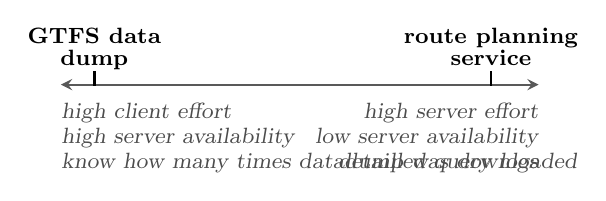
\begin{tikzpicture}[
    x=.005\textwidth,
    y=.1cm,
    axis/.style={
      line width=.8pt,
      stealth-stealth,
      color=black!65,
    },
    axislabel/.style={
      inner sep=0,
      font=\slshape\fontsize{8}{9}\selectfont,
      color=black!70,
    },
    tick/.style={
      line width=1pt,
    },
    ticklabel/.style={
      anchor=south,
      inner sep=0,
      align=center,
      font=\bfseries\fontsize{8}{8}\selectfont,
      text depth=0pt,
    },
  ]
    \newcommand\tick[2]{%
      \draw[tick] (#1, 1.7) -- (#1, -.4pt);
      \node[ticklabel] at (#1, 2.4) {#2};
    }
    \newcommand\vaguetick[1]{%
      \draw[tick,densely dotted] (#1, 1.7) -- (#1, -.4pt);
    }

    \draw[axis] (-100, 0) -- (0, 0);
    \node[axislabel,align=left,anchor=north west] at (-100, -2.3)
    {
%      generic requests\\
      high client effort\\
      high server availability\\
      know how many times datadump was downloaded
    };
    \node[axislabel,align=right,anchor=north east] at (0, -2.3)
    {
%      specific requests\\
      high server effort\\
      low server availability\\
      detailled query logs
    };

    \tick{-93}{GTFS data\\dump}
    \tick{-10}{route planning\\service}
%    \tick{-32}{Linked\\Connections}

   % \vaguetick{-84}
   % \vaguetick{-52}
   % \vaguetick{  5}
   % \vaguetick{-10}
   % \vaguetick{ 28}
   % \vaguetick{ 55}

   %\node[align=center,font=\fontsize{8}{9}\selectfont\bfseries] at (0, -8.3)
   %   {various types of\\Linked Data Fragments};
  \end{tikzpicture}
  \caption{
    This axis illustrates two extremes. With GTFS data dumps, the data reusers do all the work, and no query logs can be used. With route planning services, the servers need to do all the work, yet detailled query logs can be studied.
  }
  \label{fig:LDFAxis1}
\end{figure}

% END AXIS

The \emph{iRail} project\footnote{\url{http://hello.irail.be}} is a project started in 2008 to make the data of the Belgian railway accessible for developers.
Ever since, the project offers developer both a GTFS data dump for third party apps and a route planning API.
The API, during 2013/2014, got an average of 3000 route planning requests a day.
In this paper, we study these logs and see whether we can find interesting pattern in it.
Finally, we look at Linked Connections~\cite{lc} and whether we would still be able to have an indication of the transit flows with a Linked Data Fragments approach.

\section{Gathering the logs}
\label{sec:logs}

The logs are available at \ldots

\section{Looking for patterns}
\label{sec:method}


\section{Results}
\label{sec:results}

\todo{add a couple of nice images with explanation here}

\subsection{Pattern 1: ...}
\label{sec:pattern1}

\subsection{Pattern 2: ...}
\label{sec:pattern2}

\subsection{Pattern 3: ...}
\label{sec:pattern3}

\section{Publishing transport data}

Thoughts on publishing transport data on the web and query logs in the case of GTFS, Linked Connections\cite{lc} (linked data fragments\cite{ldf}) and webservices.

\section{Conclusion}
\label{sec:conclusion}

Query logs are very interesting

% Fix spacing after References header (as line 1308 of sig-alternate.cls breaks it)
\let\oldsection\section
\renewcommand{\section}[2][1]{\oldsection{#1}\vspace{-3pt}}

\bibliographystyle{abbrv}
\bibliography{refs}
\end{document}
